\input{../../../.preambles/02-lab_work}
\newgeometry{top=1.5cm, bottom=1.5cm, left=1cm, right=1cm}
\begin{document}
    \begin{table}[h!]
        \center
        \begin{tabular}{|C{.5}|C{.2}|C{.25}|}
            \hline
            \multicolumn{1}{|c|}{\multirow{4}{*}{Лабораторная работа № 1}} &
            Студент, группа & {{ student }}, Ф-369 \\ \cline{2-3}
            & Дата выполнения &  \\ \cline{2-3}
            & Подпись &  \\ \cline{2-3}
            Определение температуры катода и & Дата отчёта & \\ \cline{2-3}
            работы выхода материала катода & Оценка &  \\ \cline{2-3}
            & Подпись &  \\ \hline
        \end{tabular}
    \end{table}

    \emph{Цель работы:} изучение явления термоэлектронной эмиссии. Нахождение с
    помощью закона Ричардсона-Дэшмана температуры катода и работы выхода
    материала катода.
    \begin{figure}[h]
        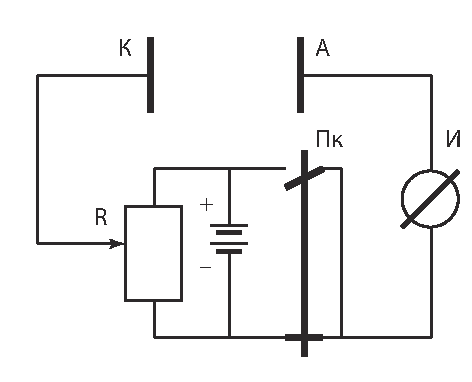
\includegraphics[width=.4\textwidth]{scheme}
    \end{figure} 
    \begin{table}[ht]
        \center
        \caption{Определение температуры катода}
        \begin{tabular}{|*{2}{C{0.08}|}*{10}{C{.04}|}} \hline
            \multirow{2}{*}{\( U_\textit{н} =\)\ \ \ \ В} &
            \( I_\textit{А},\) мкА &&&&&&&&&&\\ \cline{2-12}
            & \( U_\textit{А},\) В &&&&&&&&&&\\ \hline
            \multirow{2}{*}{\( U_\textit{н} =\)\ \ \ \ В} &
            \( I_\textit{А},\) мкА &&&&&&&&&&\\ \cline{2-12}
            & \( U_\textit{А},\) В &&&&&&&&&&\\ \hline
            \multirow{2}{*}{\( U_\textit{н} =\)\ \ \ \ В} &
            \( I_\textit{А},\) мкА &&&&&&&&&&\\ \cline{2-12}
            & \( U_\textit{А},\) В &&&&&&&&&&\\ \hline
            \multirow{2}{*}{\( U_\textit{н} =\)\ \ \ \ В} &
            \( I_\textit{А},\) мкА &&&&&&&&&&\\ \cline{2-12}
                                       & \( U_\textit{А},\) В &&&&&&&&&&\\ \hline
            \multirow{2}{*}{\( U_\textit{н} =\)\ \ \ \ В} &
            \( I_\textit{А},\) мкА &&&&&&&&&&\\ \cline{2-12}
                                       & \( U_\textit{А},\) В &&&&&&&&&&\\ \hline
            \multirow{2}{*}{\( U_\textit{н} =\)\ \ \ \ В} &
            \( I_\textit{А},\) мкА &&&&&&&&&&\\ \cline{2-12}
                                       & \( U_\textit{А},\) В &&&&&&&&&&\\ \hline
        \end{tabular}
    \end{table}
    \begin{table}[h!]
        \center
        \caption{Определение работы выхода}
        \begin{tabular}{|*{7}{C{0.1}|}}\hline
            \(T,\ K\)&&&&&&\\ \hline
            \(I_\textit{А},\ \text{мкА}\)&&&&&&\\ \hline
            \(\ln(I_\textit{А})\)&&&&&&\\ \hline
            
        \end{tabular}
    \end{table}

    \emph{Вывод:}
\end{document}
